\documentclass[11pt]{article}

    \usepackage[breakable]{tcolorbox}
    \usepackage{parskip} % Stop auto-indenting (to mimic markdown behaviour)
    

    % Basic figure setup, for now with no caption control since it's done
    % automatically by Pandoc (which extracts ![](path) syntax from Markdown).
    \usepackage{graphicx}
    % Keep aspect ratio if custom image width or height is specified
    \setkeys{Gin}{keepaspectratio}
    % Maintain compatibility with old templates. Remove in nbconvert 6.0
    \let\Oldincludegraphics\includegraphics
    % Ensure that by default, figures have no caption (until we provide a
    % proper Figure object with a Caption API and a way to capture that
    % in the conversion process - todo).
    \usepackage{caption}
    \DeclareCaptionFormat{nocaption}{}
    \captionsetup{format=nocaption,aboveskip=0pt,belowskip=0pt}

    \usepackage{float}
    \floatplacement{figure}{H} % forces figures to be placed at the correct location
    \usepackage{xcolor} % Allow colors to be defined
    \usepackage{enumerate} % Needed for markdown enumerations to work
    \usepackage{geometry} % Used to adjust the document margins
    \usepackage{amsmath} % Equations
    \usepackage{amssymb} % Equations
    \usepackage{textcomp} % defines textquotesingle
    % Hack from http://tex.stackexchange.com/a/47451/13684:
    \AtBeginDocument{%
        \def\PYZsq{\textquotesingle}% Upright quotes in Pygmentized code
    }
    \usepackage{upquote} % Upright quotes for verbatim code
    \usepackage{eurosym} % defines \euro

    \usepackage{iftex}
    \ifPDFTeX
        \usepackage[T1]{fontenc}
        \IfFileExists{alphabeta.sty}{
              \usepackage{alphabeta}
          }{
              \usepackage[mathletters]{ucs}
              \usepackage[utf8x]{inputenc}
          }
    \else
        \usepackage{fontspec}
        \usepackage{unicode-math}
    \fi

    \usepackage{fancyvrb} % verbatim replacement that allows latex
    \usepackage{grffile} % extends the file name processing of package graphics
                         % to support a larger range
    \makeatletter % fix for old versions of grffile with XeLaTeX
    \@ifpackagelater{grffile}{2019/11/01}
    {
      % Do nothing on new versions
    }
    {
      \def\Gread@@xetex#1{%
        \IfFileExists{"\Gin@base".bb}%
        {\Gread@eps{\Gin@base.bb}}%
        {\Gread@@xetex@aux#1}%
      }
    }
    \makeatother
    \usepackage[Export]{adjustbox} % Used to constrain images to a maximum size
    \adjustboxset{max size={0.9\linewidth}{0.9\paperheight}}

    % The hyperref package gives us a pdf with properly built
    % internal navigation ('pdf bookmarks' for the table of contents,
    % internal cross-reference links, web links for URLs, etc.)
    \usepackage{hyperref}
    % The default LaTeX title has an obnoxious amount of whitespace. By default,
    % titling removes some of it. It also provides customization options.
    \usepackage{titling}
    \usepackage{longtable} % longtable support required by pandoc >1.10
    \usepackage{booktabs}  % table support for pandoc > 1.12.2
    \usepackage{array}     % table support for pandoc >= 2.11.3
    \usepackage{calc}      % table minipage width calculation for pandoc >= 2.11.1
    \usepackage[inline]{enumitem} % IRkernel/repr support (it uses the enumerate* environment)
    \usepackage[normalem]{ulem} % ulem is needed to support strikethroughs (\sout)
                                % normalem makes italics be italics, not underlines
    \usepackage{soul}      % strikethrough (\st) support for pandoc >= 3.0.0
    \usepackage{mathrsfs}
    

    
    % Colors for the hyperref package
    \definecolor{urlcolor}{rgb}{0,.145,.698}
    \definecolor{linkcolor}{rgb}{.71,0.21,0.01}
    \definecolor{citecolor}{rgb}{.12,.54,.11}

    % ANSI colors
    \definecolor{ansi-black}{HTML}{3E424D}
    \definecolor{ansi-black-intense}{HTML}{282C36}
    \definecolor{ansi-red}{HTML}{E75C58}
    \definecolor{ansi-red-intense}{HTML}{B22B31}
    \definecolor{ansi-green}{HTML}{00A250}
    \definecolor{ansi-green-intense}{HTML}{007427}
    \definecolor{ansi-yellow}{HTML}{DDB62B}
    \definecolor{ansi-yellow-intense}{HTML}{B27D12}
    \definecolor{ansi-blue}{HTML}{208FFB}
    \definecolor{ansi-blue-intense}{HTML}{0065CA}
    \definecolor{ansi-magenta}{HTML}{D160C4}
    \definecolor{ansi-magenta-intense}{HTML}{A03196}
    \definecolor{ansi-cyan}{HTML}{60C6C8}
    \definecolor{ansi-cyan-intense}{HTML}{258F8F}
    \definecolor{ansi-white}{HTML}{C5C1B4}
    \definecolor{ansi-white-intense}{HTML}{A1A6B2}
    \definecolor{ansi-default-inverse-fg}{HTML}{FFFFFF}
    \definecolor{ansi-default-inverse-bg}{HTML}{000000}

    % common color for the border for error outputs.
    \definecolor{outerrorbackground}{HTML}{FFDFDF}

    % commands and environments needed by pandoc snippets
    % extracted from the output of `pandoc -s`
    \providecommand{\tightlist}{%
      \setlength{\itemsep}{0pt}\setlength{\parskip}{0pt}}
    \DefineVerbatimEnvironment{Highlighting}{Verbatim}{commandchars=\\\{\}}
    % Add ',fontsize=\small' for more characters per line
    \newenvironment{Shaded}{}{}
    \newcommand{\KeywordTok}[1]{\textcolor[rgb]{0.00,0.44,0.13}{\textbf{{#1}}}}
    \newcommand{\DataTypeTok}[1]{\textcolor[rgb]{0.56,0.13,0.00}{{#1}}}
    \newcommand{\DecValTok}[1]{\textcolor[rgb]{0.25,0.63,0.44}{{#1}}}
    \newcommand{\BaseNTok}[1]{\textcolor[rgb]{0.25,0.63,0.44}{{#1}}}
    \newcommand{\FloatTok}[1]{\textcolor[rgb]{0.25,0.63,0.44}{{#1}}}
    \newcommand{\CharTok}[1]{\textcolor[rgb]{0.25,0.44,0.63}{{#1}}}
    \newcommand{\StringTok}[1]{\textcolor[rgb]{0.25,0.44,0.63}{{#1}}}
    \newcommand{\CommentTok}[1]{\textcolor[rgb]{0.38,0.63,0.69}{\textit{{#1}}}}
    \newcommand{\OtherTok}[1]{\textcolor[rgb]{0.00,0.44,0.13}{{#1}}}
    \newcommand{\AlertTok}[1]{\textcolor[rgb]{1.00,0.00,0.00}{\textbf{{#1}}}}
    \newcommand{\FunctionTok}[1]{\textcolor[rgb]{0.02,0.16,0.49}{{#1}}}
    \newcommand{\RegionMarkerTok}[1]{{#1}}
    \newcommand{\ErrorTok}[1]{\textcolor[rgb]{1.00,0.00,0.00}{\textbf{{#1}}}}
    \newcommand{\NormalTok}[1]{{#1}}

    % Additional commands for more recent versions of Pandoc
    \newcommand{\ConstantTok}[1]{\textcolor[rgb]{0.53,0.00,0.00}{{#1}}}
    \newcommand{\SpecialCharTok}[1]{\textcolor[rgb]{0.25,0.44,0.63}{{#1}}}
    \newcommand{\VerbatimStringTok}[1]{\textcolor[rgb]{0.25,0.44,0.63}{{#1}}}
    \newcommand{\SpecialStringTok}[1]{\textcolor[rgb]{0.73,0.40,0.53}{{#1}}}
    \newcommand{\ImportTok}[1]{{#1}}
    \newcommand{\DocumentationTok}[1]{\textcolor[rgb]{0.73,0.13,0.13}{\textit{{#1}}}}
    \newcommand{\AnnotationTok}[1]{\textcolor[rgb]{0.38,0.63,0.69}{\textbf{\textit{{#1}}}}}
    \newcommand{\CommentVarTok}[1]{\textcolor[rgb]{0.38,0.63,0.69}{\textbf{\textit{{#1}}}}}
    \newcommand{\VariableTok}[1]{\textcolor[rgb]{0.10,0.09,0.49}{{#1}}}
    \newcommand{\ControlFlowTok}[1]{\textcolor[rgb]{0.00,0.44,0.13}{\textbf{{#1}}}}
    \newcommand{\OperatorTok}[1]{\textcolor[rgb]{0.40,0.40,0.40}{{#1}}}
    \newcommand{\BuiltInTok}[1]{{#1}}
    \newcommand{\ExtensionTok}[1]{{#1}}
    \newcommand{\PreprocessorTok}[1]{\textcolor[rgb]{0.74,0.48,0.00}{{#1}}}
    \newcommand{\AttributeTok}[1]{\textcolor[rgb]{0.49,0.56,0.16}{{#1}}}
    \newcommand{\InformationTok}[1]{\textcolor[rgb]{0.38,0.63,0.69}{\textbf{\textit{{#1}}}}}
    \newcommand{\WarningTok}[1]{\textcolor[rgb]{0.38,0.63,0.69}{\textbf{\textit{{#1}}}}}
    \makeatletter
    \newsavebox\pandoc@box
    \newcommand*\pandocbounded[1]{%
      \sbox\pandoc@box{#1}%
      % scaling factors for width and height
      \Gscale@div\@tempa\textheight{\dimexpr\ht\pandoc@box+\dp\pandoc@box\relax}%
      \Gscale@div\@tempb\linewidth{\wd\pandoc@box}%
      % select the smaller of both
      \ifdim\@tempb\p@<\@tempa\p@
        \let\@tempa\@tempb
      \fi
      % scaling accordingly (\@tempa < 1)
      \ifdim\@tempa\p@<\p@
        \scalebox{\@tempa}{\usebox\pandoc@box}%
      % scaling not needed, use as it is
      \else
        \usebox{\pandoc@box}%
      \fi
    }
    \makeatother

    % Define a nice break command that doesn't care if a line doesn't already
    % exist.
    \def\br{\hspace*{\fill} \\* }
    % Math Jax compatibility definitions
    \def\gt{>}
    \def\lt{<}
    \let\Oldtex\TeX
    \let\Oldlatex\LaTeX
    \renewcommand{\TeX}{\textrm{\Oldtex}}
    \renewcommand{\LaTeX}{\textrm{\Oldlatex}}
    % Document parameters
    % Document title
    \title{02\_notes}
    
    
    
    
    
    
    
% Pygments definitions
\makeatletter
\def\PY@reset{\let\PY@it=\relax \let\PY@bf=\relax%
    \let\PY@ul=\relax \let\PY@tc=\relax%
    \let\PY@bc=\relax \let\PY@ff=\relax}
\def\PY@tok#1{\csname PY@tok@#1\endcsname}
\def\PY@toks#1+{\ifx\relax#1\empty\else%
    \PY@tok{#1}\expandafter\PY@toks\fi}
\def\PY@do#1{\PY@bc{\PY@tc{\PY@ul{%
    \PY@it{\PY@bf{\PY@ff{#1}}}}}}}
\def\PY#1#2{\PY@reset\PY@toks#1+\relax+\PY@do{#2}}

\@namedef{PY@tok@w}{\def\PY@tc##1{\textcolor[rgb]{0.73,0.73,0.73}{##1}}}
\@namedef{PY@tok@c}{\let\PY@it=\textit\def\PY@tc##1{\textcolor[rgb]{0.24,0.48,0.48}{##1}}}
\@namedef{PY@tok@cp}{\def\PY@tc##1{\textcolor[rgb]{0.61,0.40,0.00}{##1}}}
\@namedef{PY@tok@k}{\let\PY@bf=\textbf\def\PY@tc##1{\textcolor[rgb]{0.00,0.50,0.00}{##1}}}
\@namedef{PY@tok@kp}{\def\PY@tc##1{\textcolor[rgb]{0.00,0.50,0.00}{##1}}}
\@namedef{PY@tok@kt}{\def\PY@tc##1{\textcolor[rgb]{0.69,0.00,0.25}{##1}}}
\@namedef{PY@tok@o}{\def\PY@tc##1{\textcolor[rgb]{0.40,0.40,0.40}{##1}}}
\@namedef{PY@tok@ow}{\let\PY@bf=\textbf\def\PY@tc##1{\textcolor[rgb]{0.67,0.13,1.00}{##1}}}
\@namedef{PY@tok@nb}{\def\PY@tc##1{\textcolor[rgb]{0.00,0.50,0.00}{##1}}}
\@namedef{PY@tok@nf}{\def\PY@tc##1{\textcolor[rgb]{0.00,0.00,1.00}{##1}}}
\@namedef{PY@tok@nc}{\let\PY@bf=\textbf\def\PY@tc##1{\textcolor[rgb]{0.00,0.00,1.00}{##1}}}
\@namedef{PY@tok@nn}{\let\PY@bf=\textbf\def\PY@tc##1{\textcolor[rgb]{0.00,0.00,1.00}{##1}}}
\@namedef{PY@tok@ne}{\let\PY@bf=\textbf\def\PY@tc##1{\textcolor[rgb]{0.80,0.25,0.22}{##1}}}
\@namedef{PY@tok@nv}{\def\PY@tc##1{\textcolor[rgb]{0.10,0.09,0.49}{##1}}}
\@namedef{PY@tok@no}{\def\PY@tc##1{\textcolor[rgb]{0.53,0.00,0.00}{##1}}}
\@namedef{PY@tok@nl}{\def\PY@tc##1{\textcolor[rgb]{0.46,0.46,0.00}{##1}}}
\@namedef{PY@tok@ni}{\let\PY@bf=\textbf\def\PY@tc##1{\textcolor[rgb]{0.44,0.44,0.44}{##1}}}
\@namedef{PY@tok@na}{\def\PY@tc##1{\textcolor[rgb]{0.41,0.47,0.13}{##1}}}
\@namedef{PY@tok@nt}{\let\PY@bf=\textbf\def\PY@tc##1{\textcolor[rgb]{0.00,0.50,0.00}{##1}}}
\@namedef{PY@tok@nd}{\def\PY@tc##1{\textcolor[rgb]{0.67,0.13,1.00}{##1}}}
\@namedef{PY@tok@s}{\def\PY@tc##1{\textcolor[rgb]{0.73,0.13,0.13}{##1}}}
\@namedef{PY@tok@sd}{\let\PY@it=\textit\def\PY@tc##1{\textcolor[rgb]{0.73,0.13,0.13}{##1}}}
\@namedef{PY@tok@si}{\let\PY@bf=\textbf\def\PY@tc##1{\textcolor[rgb]{0.64,0.35,0.47}{##1}}}
\@namedef{PY@tok@se}{\let\PY@bf=\textbf\def\PY@tc##1{\textcolor[rgb]{0.67,0.36,0.12}{##1}}}
\@namedef{PY@tok@sr}{\def\PY@tc##1{\textcolor[rgb]{0.64,0.35,0.47}{##1}}}
\@namedef{PY@tok@ss}{\def\PY@tc##1{\textcolor[rgb]{0.10,0.09,0.49}{##1}}}
\@namedef{PY@tok@sx}{\def\PY@tc##1{\textcolor[rgb]{0.00,0.50,0.00}{##1}}}
\@namedef{PY@tok@m}{\def\PY@tc##1{\textcolor[rgb]{0.40,0.40,0.40}{##1}}}
\@namedef{PY@tok@gh}{\let\PY@bf=\textbf\def\PY@tc##1{\textcolor[rgb]{0.00,0.00,0.50}{##1}}}
\@namedef{PY@tok@gu}{\let\PY@bf=\textbf\def\PY@tc##1{\textcolor[rgb]{0.50,0.00,0.50}{##1}}}
\@namedef{PY@tok@gd}{\def\PY@tc##1{\textcolor[rgb]{0.63,0.00,0.00}{##1}}}
\@namedef{PY@tok@gi}{\def\PY@tc##1{\textcolor[rgb]{0.00,0.52,0.00}{##1}}}
\@namedef{PY@tok@gr}{\def\PY@tc##1{\textcolor[rgb]{0.89,0.00,0.00}{##1}}}
\@namedef{PY@tok@ge}{\let\PY@it=\textit}
\@namedef{PY@tok@gs}{\let\PY@bf=\textbf}
\@namedef{PY@tok@ges}{\let\PY@bf=\textbf\let\PY@it=\textit}
\@namedef{PY@tok@gp}{\let\PY@bf=\textbf\def\PY@tc##1{\textcolor[rgb]{0.00,0.00,0.50}{##1}}}
\@namedef{PY@tok@go}{\def\PY@tc##1{\textcolor[rgb]{0.44,0.44,0.44}{##1}}}
\@namedef{PY@tok@gt}{\def\PY@tc##1{\textcolor[rgb]{0.00,0.27,0.87}{##1}}}
\@namedef{PY@tok@err}{\def\PY@bc##1{{\setlength{\fboxsep}{\string -\fboxrule}\fcolorbox[rgb]{1.00,0.00,0.00}{1,1,1}{\strut ##1}}}}
\@namedef{PY@tok@kc}{\let\PY@bf=\textbf\def\PY@tc##1{\textcolor[rgb]{0.00,0.50,0.00}{##1}}}
\@namedef{PY@tok@kd}{\let\PY@bf=\textbf\def\PY@tc##1{\textcolor[rgb]{0.00,0.50,0.00}{##1}}}
\@namedef{PY@tok@kn}{\let\PY@bf=\textbf\def\PY@tc##1{\textcolor[rgb]{0.00,0.50,0.00}{##1}}}
\@namedef{PY@tok@kr}{\let\PY@bf=\textbf\def\PY@tc##1{\textcolor[rgb]{0.00,0.50,0.00}{##1}}}
\@namedef{PY@tok@bp}{\def\PY@tc##1{\textcolor[rgb]{0.00,0.50,0.00}{##1}}}
\@namedef{PY@tok@fm}{\def\PY@tc##1{\textcolor[rgb]{0.00,0.00,1.00}{##1}}}
\@namedef{PY@tok@vc}{\def\PY@tc##1{\textcolor[rgb]{0.10,0.09,0.49}{##1}}}
\@namedef{PY@tok@vg}{\def\PY@tc##1{\textcolor[rgb]{0.10,0.09,0.49}{##1}}}
\@namedef{PY@tok@vi}{\def\PY@tc##1{\textcolor[rgb]{0.10,0.09,0.49}{##1}}}
\@namedef{PY@tok@vm}{\def\PY@tc##1{\textcolor[rgb]{0.10,0.09,0.49}{##1}}}
\@namedef{PY@tok@sa}{\def\PY@tc##1{\textcolor[rgb]{0.73,0.13,0.13}{##1}}}
\@namedef{PY@tok@sb}{\def\PY@tc##1{\textcolor[rgb]{0.73,0.13,0.13}{##1}}}
\@namedef{PY@tok@sc}{\def\PY@tc##1{\textcolor[rgb]{0.73,0.13,0.13}{##1}}}
\@namedef{PY@tok@dl}{\def\PY@tc##1{\textcolor[rgb]{0.73,0.13,0.13}{##1}}}
\@namedef{PY@tok@s2}{\def\PY@tc##1{\textcolor[rgb]{0.73,0.13,0.13}{##1}}}
\@namedef{PY@tok@sh}{\def\PY@tc##1{\textcolor[rgb]{0.73,0.13,0.13}{##1}}}
\@namedef{PY@tok@s1}{\def\PY@tc##1{\textcolor[rgb]{0.73,0.13,0.13}{##1}}}
\@namedef{PY@tok@mb}{\def\PY@tc##1{\textcolor[rgb]{0.40,0.40,0.40}{##1}}}
\@namedef{PY@tok@mf}{\def\PY@tc##1{\textcolor[rgb]{0.40,0.40,0.40}{##1}}}
\@namedef{PY@tok@mh}{\def\PY@tc##1{\textcolor[rgb]{0.40,0.40,0.40}{##1}}}
\@namedef{PY@tok@mi}{\def\PY@tc##1{\textcolor[rgb]{0.40,0.40,0.40}{##1}}}
\@namedef{PY@tok@il}{\def\PY@tc##1{\textcolor[rgb]{0.40,0.40,0.40}{##1}}}
\@namedef{PY@tok@mo}{\def\PY@tc##1{\textcolor[rgb]{0.40,0.40,0.40}{##1}}}
\@namedef{PY@tok@ch}{\let\PY@it=\textit\def\PY@tc##1{\textcolor[rgb]{0.24,0.48,0.48}{##1}}}
\@namedef{PY@tok@cm}{\let\PY@it=\textit\def\PY@tc##1{\textcolor[rgb]{0.24,0.48,0.48}{##1}}}
\@namedef{PY@tok@cpf}{\let\PY@it=\textit\def\PY@tc##1{\textcolor[rgb]{0.24,0.48,0.48}{##1}}}
\@namedef{PY@tok@c1}{\let\PY@it=\textit\def\PY@tc##1{\textcolor[rgb]{0.24,0.48,0.48}{##1}}}
\@namedef{PY@tok@cs}{\let\PY@it=\textit\def\PY@tc##1{\textcolor[rgb]{0.24,0.48,0.48}{##1}}}

\def\PYZbs{\char`\\}
\def\PYZus{\char`\_}
\def\PYZob{\char`\{}
\def\PYZcb{\char`\}}
\def\PYZca{\char`\^}
\def\PYZam{\char`\&}
\def\PYZlt{\char`\<}
\def\PYZgt{\char`\>}
\def\PYZsh{\char`\#}
\def\PYZpc{\char`\%}
\def\PYZdl{\char`\$}
\def\PYZhy{\char`\-}
\def\PYZsq{\char`\'}
\def\PYZdq{\char`\"}
\def\PYZti{\char`\~}
% for compatibility with earlier versions
\def\PYZat{@}
\def\PYZlb{[}
\def\PYZrb{]}
\makeatother


    % For linebreaks inside Verbatim environment from package fancyvrb.
    \makeatletter
        \newbox\Wrappedcontinuationbox
        \newbox\Wrappedvisiblespacebox
        \newcommand*\Wrappedvisiblespace {\textcolor{red}{\textvisiblespace}}
        \newcommand*\Wrappedcontinuationsymbol {\textcolor{red}{\llap{\tiny$\m@th\hookrightarrow$}}}
        \newcommand*\Wrappedcontinuationindent {3ex }
        \newcommand*\Wrappedafterbreak {\kern\Wrappedcontinuationindent\copy\Wrappedcontinuationbox}
        % Take advantage of the already applied Pygments mark-up to insert
        % potential linebreaks for TeX processing.
        %        {, <, #, %, $, ' and ": go to next line.
        %        _, }, ^, &, >, - and ~: stay at end of broken line.
        % Use of \textquotesingle for straight quote.
        \newcommand*\Wrappedbreaksatspecials {%
            \def\PYGZus{\discretionary{\char`\_}{\Wrappedafterbreak}{\char`\_}}%
            \def\PYGZob{\discretionary{}{\Wrappedafterbreak\char`\{}{\char`\{}}%
            \def\PYGZcb{\discretionary{\char`\}}{\Wrappedafterbreak}{\char`\}}}%
            \def\PYGZca{\discretionary{\char`\^}{\Wrappedafterbreak}{\char`\^}}%
            \def\PYGZam{\discretionary{\char`\&}{\Wrappedafterbreak}{\char`\&}}%
            \def\PYGZlt{\discretionary{}{\Wrappedafterbreak\char`\<}{\char`\<}}%
            \def\PYGZgt{\discretionary{\char`\>}{\Wrappedafterbreak}{\char`\>}}%
            \def\PYGZsh{\discretionary{}{\Wrappedafterbreak\char`\#}{\char`\#}}%
            \def\PYGZpc{\discretionary{}{\Wrappedafterbreak\char`\%}{\char`\%}}%
            \def\PYGZdl{\discretionary{}{\Wrappedafterbreak\char`\$}{\char`\$}}%
            \def\PYGZhy{\discretionary{\char`\-}{\Wrappedafterbreak}{\char`\-}}%
            \def\PYGZsq{\discretionary{}{\Wrappedafterbreak\textquotesingle}{\textquotesingle}}%
            \def\PYGZdq{\discretionary{}{\Wrappedafterbreak\char`\"}{\char`\"}}%
            \def\PYGZti{\discretionary{\char`\~}{\Wrappedafterbreak}{\char`\~}}%
        }
        % Some characters . , ; ? ! / are not pygmentized.
        % This macro makes them "active" and they will insert potential linebreaks
        \newcommand*\Wrappedbreaksatpunct {%
            \lccode`\~`\.\lowercase{\def~}{\discretionary{\hbox{\char`\.}}{\Wrappedafterbreak}{\hbox{\char`\.}}}%
            \lccode`\~`\,\lowercase{\def~}{\discretionary{\hbox{\char`\,}}{\Wrappedafterbreak}{\hbox{\char`\,}}}%
            \lccode`\~`\;\lowercase{\def~}{\discretionary{\hbox{\char`\;}}{\Wrappedafterbreak}{\hbox{\char`\;}}}%
            \lccode`\~`\:\lowercase{\def~}{\discretionary{\hbox{\char`\:}}{\Wrappedafterbreak}{\hbox{\char`\:}}}%
            \lccode`\~`\?\lowercase{\def~}{\discretionary{\hbox{\char`\?}}{\Wrappedafterbreak}{\hbox{\char`\?}}}%
            \lccode`\~`\!\lowercase{\def~}{\discretionary{\hbox{\char`\!}}{\Wrappedafterbreak}{\hbox{\char`\!}}}%
            \lccode`\~`\/\lowercase{\def~}{\discretionary{\hbox{\char`\/}}{\Wrappedafterbreak}{\hbox{\char`\/}}}%
            \catcode`\.\active
            \catcode`\,\active
            \catcode`\;\active
            \catcode`\:\active
            \catcode`\?\active
            \catcode`\!\active
            \catcode`\/\active
            \lccode`\~`\~
        }
    \makeatother

    \let\OriginalVerbatim=\Verbatim
    \makeatletter
    \renewcommand{\Verbatim}[1][1]{%
        %\parskip\z@skip
        \sbox\Wrappedcontinuationbox {\Wrappedcontinuationsymbol}%
        \sbox\Wrappedvisiblespacebox {\FV@SetupFont\Wrappedvisiblespace}%
        \def\FancyVerbFormatLine ##1{\hsize\linewidth
            \vtop{\raggedright\hyphenpenalty\z@\exhyphenpenalty\z@
                \doublehyphendemerits\z@\finalhyphendemerits\z@
                \strut ##1\strut}%
        }%
        % If the linebreak is at a space, the latter will be displayed as visible
        % space at end of first line, and a continuation symbol starts next line.
        % Stretch/shrink are however usually zero for typewriter font.
        \def\FV@Space {%
            \nobreak\hskip\z@ plus\fontdimen3\font minus\fontdimen4\font
            \discretionary{\copy\Wrappedvisiblespacebox}{\Wrappedafterbreak}
            {\kern\fontdimen2\font}%
        }%

        % Allow breaks at special characters using \PYG... macros.
        \Wrappedbreaksatspecials
        % Breaks at punctuation characters . , ; ? ! and / need catcode=\active
        \OriginalVerbatim[#1,codes*=\Wrappedbreaksatpunct]%
    }
    \makeatother

    % Exact colors from NB
    \definecolor{incolor}{HTML}{303F9F}
    \definecolor{outcolor}{HTML}{D84315}
    \definecolor{cellborder}{HTML}{CFCFCF}
    \definecolor{cellbackground}{HTML}{F7F7F7}

    % prompt
    \makeatletter
    \newcommand{\boxspacing}{\kern\kvtcb@left@rule\kern\kvtcb@boxsep}
    \makeatother
    \newcommand{\prompt}[4]{
        {\ttfamily\llap{{\color{#2}[#3]:\hspace{3pt}#4}}\vspace{-\baselineskip}}
    }
    

    
    % Prevent overflowing lines due to hard-to-break entities
    \sloppy
    % Setup hyperref package
    \hypersetup{
      breaklinks=true,  % so long urls are correctly broken across lines
      colorlinks=true,
      urlcolor=urlcolor,
      linkcolor=linkcolor,
      citecolor=citecolor,
      }
    % Slightly bigger margins than the latex defaults
    
    \geometry{verbose,tmargin=1in,bmargin=1in,lmargin=1in,rmargin=1in}
    
    

\begin{document}
    
    \maketitle
    
    

    
    \section{Week 2 - Notes: Mathematical
Preliminaries}\label{week-2---notes-mathematical-preliminaries}

We need a few things to get us started with making models of classical
phenomenon. A few of those topics might be familiar to you; things like
vectors, and derivatives. But we'll also need to introduce some new
concepts, like the concept of
\href{https://en.wikipedia.org/wiki/Discretization}{Discretization}. In
particular, we will introduce a powerful method for solving all forms of
Differential Equations -- Euler-Cromer Integration. We start by
introducing the concept of Euler Discretization, and then we'll move on
to Euler-Cromer Integration later in the course.

    \subsection{Euler Discretization}\label{euler-discretization}

Another useful formulation of Classical Mechanics uses discrete points
in time to make approximate predictions of the motion. This is called
the \href{https://en.wikipedia.org/wiki/Euler_method}{Euler Method}. The
Euler Method is a simple numerical method to solve ordinary differential
equations. The method is based on the idea of approximating the
derivative of a function by a finite difference.

We posit discrete time, like snapshots of the motion where a given
measure of time \(t_i\) exists in a discrete set of times between
\(t_0\) and \(t_f\). That is,
\(t_i \in \{t_0, t_1, t_2, \ldots, t_f\}\). We conceive of the motion as
discrete like the points in the figure below.

In this case, the points are equally spaced in time, such that
\(t_{i+1} - t_i = \Delta t\). This gives a simple table of the motion of
the object at each time step:

\begin{longtable}[]{@{}ll@{}}
\toprule\noalign{}
time & position \\
\midrule\noalign{}
\endhead
\bottomrule\noalign{}
\endlastfoot
\(t_0\) & \(y_0\) \\
\(t_1\) & \(y_1\) \\
\(t_2\) & \(y_2\) \\
\(\ldots\) & \(\ldots\) \\
\end{longtable}

where \(y_i\) is the position of the object at time \(t_i\). Here,
\(t_i = t_0 + i\Delta t\) -- equal time spacing -- and \(y(t_i) = y_i\)
indicates the position of the object at time \(t_i\).

\subsubsection{Predicting the Motion}\label{predicting-the-motion}

This formulation can be used to predict the motion of the object. Let's
first define the average velocity over a time step, \(\Delta t\), like
this:

\[v(t) = \dfrac{y(t+\Delta t) - y(t)}{\Delta t}\]

Now, we know that at time, \(t_i\), the velocity is \(v_i\):
\(v(t_i) = v_i\) If we make the time step small,
\(\Delta t \rightarrow 0\), then the average velocity is approximately
the velocity at time \(t_i\). Thus, we can write the velocity at time
\(t_{i}\) as:

\[v_{i} = \dfrac{y_{i+1} - y_i}{\Delta t}\]

\textbf{Note} If we take the limit that \(\Delta t \rightarrow 0\), then
the average velocity becomes the instantaneous velocity. This stems from
the
\href{https://en.wikipedia.org/wiki/Fundamental_theorem_of_calculus}{Fundamental
Theorem of Calculus}.

\[\lim_{\Delta t \rightarrow 0} \dfrac{y(t+\Delta t) - y(t)}{\Delta t} = \dfrac{dy}{dt} = \dot{y}\]

What about the acceleration? We can use the same idea to approximate the
acceleration. The average acceleration is given by:

\[a(t) = \dfrac{v(t+\Delta t) - v(t)}{\Delta t}\]

And thus, the acceleration at time \(t_i\) is:

\[a_i = \dfrac{v_{i+1} - v_i}{\Delta t}\]

Again, if we take the limit that \(\Delta t \rightarrow 0\), then the
average acceleration becomes the instantaneous acceleration:

\[\lim_{\Delta t \rightarrow 0} \dfrac{v(t+\Delta t) - v(t)}{\Delta t} = \dfrac{dv}{dt} = \dot{v}\]

\subsubsection{Video Summary (13
minutes)}\label{video-summary-13-minutes}

There's many videos covering the topic of Euler's method. Here's a video
that covers the basics of Euler's method and how it can be used to solve
differential equations. It somewhat follows the notes above, but it's
always good to hear another perspective.

\begin{itemize}
\tightlist
\item
  Direct Link: \url{https://youtube.com/watch?v=_0mvWedqW7c}
\end{itemize}

    \begin{tcolorbox}[breakable, size=fbox, boxrule=1pt, pad at break*=1mm,colback=cellbackground, colframe=cellborder]
\prompt{In}{incolor}{2}{\boxspacing}
\begin{Verbatim}[commandchars=\\\{\}]
\PY{k+kn}{from}\PY{+w}{ }\PY{n+nn}{IPython}\PY{n+nn}{.}\PY{n+nn}{display}\PY{+w}{ }\PY{k+kn}{import} \PY{n}{YouTubeVideo}

\PY{n}{YouTubeVideo}\PY{p}{(}\PY{l+s+s1}{\PYZsq{}}\PY{l+s+s1}{\PYZus{}0mvWedqW7c}\PY{l+s+s1}{\PYZsq{}}\PY{p}{,} \PY{n}{width}\PY{o}{=}\PY{l+m+mi}{720}\PY{p}{,} \PY{n}{height}\PY{o}{=}\PY{l+m+mi}{405}\PY{p}{)}
\end{Verbatim}
\end{tcolorbox}
 
            
\prompt{Out}{outcolor}{2}{}
    
    \begin{center}
    \adjustimage{max size={0.9\linewidth}{0.9\paperheight}}{02_notes_files/02_notes_2_0.jpg}
    \end{center}
    { \hspace*{\fill} \\}
    

    \subsection{Discretizing Newton's Second
Law}\label{discretizing-newtons-second-law}

We can use the Euler Method to discretize Newton's Second Law, and this
allows us to predict the motion of the object using iterative methods.
These methods are well-suited for computers, and we will learn how to
implement them in this course.

Let there be a 1D net force acting the x-direction on an object of mass
\(m\), \(F(x)\). Here the force changes with position. We can discretize
this force as a function of position, \(F(x_i)\). The net force acting
on the object is:

\[F(x_i) = F_i\]

Using Newton's Second Law, we can write the acceleration of the object
as:

\[a_i = \dfrac{F_i}{m}\]

But the definition of the average acceleration gives:

\[a_i = \dfrac{v_{i+1} - v_i}{\Delta t}\]

Or in terms of the predicted velocity, \(v_{i+1}\):

\[v_{i+1} = v_i + a_i\Delta t\]

Or in terms of the net force:

\[v_{i+1} = v_i + \dfrac{F_i}{m}\Delta t\]

\textbf{This is the Euler formulation for predicting the velocity of the
object in the next time step -- given the velocity at the current time
step.}

We pause here and will return to this formulation later, but this
discretization is the basis for many numerical methods in classical
mechanics, and we can apply it to solve the falling object problem
above.

\subsubsection{Looking Ahead}\label{looking-ahead}

The development of the forward Euler scheme is the basis for many
numerical methods in physics, and especially in classical mechanics. The
video below is a longer introduction to the Euler Method and how it can
be used to solve differential equations. It's a bit more advanced than
the previous video, but it's a good introduction to the topic. We will
revisit this topic a number of times, and you will have a chance to
implement these methods in Python. \emph{This video will be posted again
when we cover numerical methods in more detail.}

\begin{itemize}
\tightlist
\item
  Direct Link: \url{https://www.youtube.com/watch?v=MstPeOTCVzQ}
\end{itemize}

    \begin{tcolorbox}[breakable, size=fbox, boxrule=1pt, pad at break*=1mm,colback=cellbackground, colframe=cellborder]
\prompt{In}{incolor}{3}{\boxspacing}
\begin{Verbatim}[commandchars=\\\{\}]
\PY{k+kn}{from}\PY{+w}{ }\PY{n+nn}{IPython}\PY{n+nn}{.}\PY{n+nn}{display}\PY{+w}{ }\PY{k+kn}{import} \PY{n}{YouTubeVideo}

\PY{n}{YouTubeVideo}\PY{p}{(}\PY{l+s+s1}{\PYZsq{}}\PY{l+s+s1}{MstPeOTCVzQ}\PY{l+s+s1}{\PYZsq{}}\PY{p}{,} \PY{n}{width}\PY{o}{=}\PY{l+m+mi}{720}\PY{p}{,} \PY{n}{height}\PY{o}{=}\PY{l+m+mi}{405}\PY{p}{)}
\end{Verbatim}
\end{tcolorbox}
 
            
\prompt{Out}{outcolor}{3}{}
    
    \begin{center}
    \adjustimage{max size={0.9\linewidth}{0.9\paperheight}}{02_notes_files/02_notes_4_0.jpg}
    \end{center}
    { \hspace*{\fill} \\}
    

    \subsection{Additional Mathematical
Preliminaries}\label{additional-mathematical-preliminaries}

As you have noticed, much of what we do in classical mechanics involves
solving differential equations. We will explore how to solve these
equations in this course. But also notice that most of the work involves
vector manipulation and/or decomposition. Thus, we will need to be
comfortable with vectors. Below are some mathematical concepts of
vectors that we will use in this course.

\subsubsection{Vectors and Coordinates}\label{vectors-and-coordinates}

The figure below shows a vector in two dimensions.

\begin{figure}
\centering
\pandocbounded{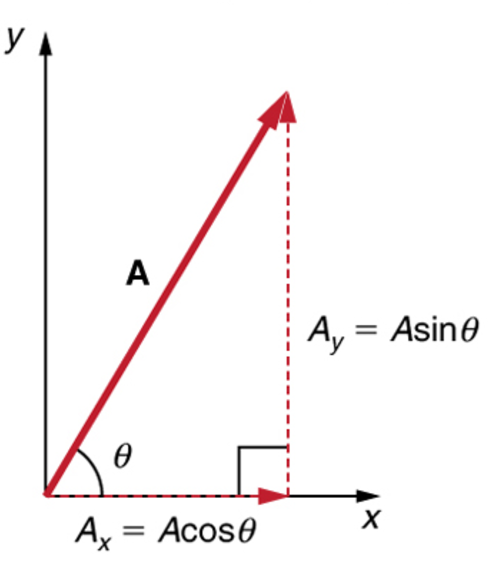
\includegraphics[keepaspectratio,alt={Vector in Two Dimensions; the vector is defined by its magnitude, A, and its direction, \textbackslash theta}]{/Users/caballero/repos/teaching/modern-classical-mechanics/images/notes/week2/2dvector.png}}
\caption{Vector in Two Dimensions; the vector is defined by its
magnitude, \(A\), and its direction, \(\theta\)}
\end{figure}

The vector is defined by its magnitude, \(A\), and its direction,
\(\theta\). The vector can be decomposed into two components, \(A_x\)
and \(A_y\), in the \(x\) and \(y\) directions, respectively.

The magnitude of the vector is given by the Pythagorean theorem:

\[|\vec{A}| = A = \sqrt{A_x^2 + A_y^2}\]

The angle of the vector is given by the tangent of the angle:

\[\theta = \tan^{-1}\left(\dfrac{A_y}{A_x}\right)\]

We can find the \emph{vector components} using the magnitude and angle:

\[A_x = A\cos(\theta)\] \[A_y = A\sin(\theta)\]

It's important to note that the vector components are the projections of
the vector onto the \(x\) and \(y\) axes. The vector components are
scalars, and the vector is a sum of the components. We can write the
vector in several common forms:

\[\vec{A} = A_x\hat{x} + A_y\hat{y}  = A_x\hat{i} + A_y\hat{j} = A_x\hat{e}_x + A_y\hat{e}_y.\]

\paragraph{Unit Vectors}\label{unit-vectors}

The unit vectors, \(\hat{x}\), \(\hat{y}\), \(\hat{i}\), \(\hat{j}\),
\(\hat{e}_x\), and \(\hat{e}_y\), are the basis vectors in the \(x\) and
\(y\) directions. The unit vectors are used to define the vector
components.

Interestingly, the angle of the vector is not needed to write the vector
in Plane Polar Coordinates (\(r\), \(\theta\)). The vector can be
written as:

\[\vec{A} = A\hat{A}\]

where \(\hat{A}\) is the unit vector in the direction of \(\vec{A}\).
Let's check that works out:

\[\vec{A} = A_x\hat{x} + A_y\hat{y}\]

\[|\vec{A}| = A = \sqrt{A_x^2 + A_y^2}\]

\[\hat{A} = \dfrac{\vec{A}}{|\vec{A}|} = \dfrac{A_x\hat{x} + A_y\hat{y}}{\sqrt{A_x^2 + A_y^2}}\]

Such that,

\[\vec{A} = A\hat{A} = A_x\hat{x} + A_y\hat{y}\]

Cartesian unit vectors are fixed in space and time when in an inertial
reference frame. However, the unit vectors in Plane Polar Coordinates
are not fixed in space and time. They rotate with the vector. This is a
common source of confusion when working with vectors in different
coordinate systems, which we will come back to later.

The magnitude of a unit vector is always one, \(|\hat{A}| = 1\). And
unit vectors are orthogonal to each other,
\(\hat{x} \cdot \hat{y} = 0\).

    \subsubsection{Multiplication of
Vectors}\label{multiplication-of-vectors}

\paragraph{Dot (Scalar) Product}\label{dot-scalar-product}

A dot product of two vectors is a scalar quantity. The dot product of
two 3D vectors, \(\vec{a}\) and \(\vec{b}\), is given by:

\[\vec{a} \cdot \vec{b} = a_xb_x + a_yb_y + a_zb_z\]

This product is also equal to the product of the magnitudes of the
vectors and the cosine of the angle between them:

\[\vec{a} \cdot \vec{b} = |\vec{a}||\vec{b}|\cos(\phi).\]

The figure below shows the relationship between the vectors and the
angle.

\begin{figure}
\centering
\pandocbounded{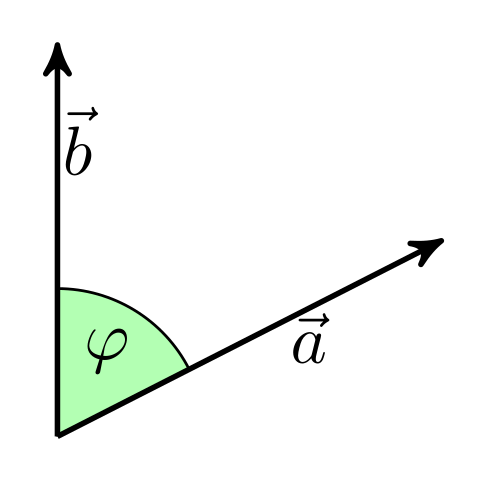
\includegraphics[keepaspectratio,alt={Dot Product of Two Vectors; the dot product is the product of the magnitudes of the vectors and the cosine of the angle between them}]{/Users/caballero/repos/teaching/modern-classical-mechanics/images/notes/week2/Dot-product.png}}
\caption{Dot Product of Two Vectors; the dot product is the product of
the magnitudes of the vectors and the cosine of the angle between them}
\end{figure}

Source:
\href{https://commons.wikimedia.org/wiki/File:Dot-product-1.svg}{Wikipedia}

Much like scalar multiplication, a dot produce is distributive:

\[\vec{a} \cdot (\vec{b} + \vec{c}) = \vec{a} \cdot \vec{b} + \vec{a} \cdot \vec{c}\]

Here's the proof:

\[\vec{a} \cdot (\vec{b} + \vec{c}) = a_x(b_x + c_x) + a_y(b_y + c_y) + a_z(b_z + c_z)\]

\[= a_xb_x + a_xc_x + a_yb_y + a_yc_y + a_zb_z + a_zc_z\]

\[= \vec{a} \cdot \vec{b} + \vec{a} \cdot \vec{c}\]

\paragraph{Cross (Vector) Product}\label{cross-vector-product}

The cross product of two vectors is a vector quantity. The cross product
of two 3D vectors, \(\vec{a}\) and \(\vec{b}\), is given by:

\[\vec{a} \times \vec{b} = \begin{vmatrix} \hat{x} & \hat{y} & \hat{z} \\ a_x & a_y & a_z \\ b_x & b_y & b_z \end{vmatrix}\]

This results in a vector that has the following components:

\[\vec{a} \times \vec{b} = (a_yb_z - a_zb_y)\hat{x} - (a_xb_z-a_zb_x)\hat{y} + (a_xb_y - a_yb_x)\hat{z}\]

A few notes about cross products:

\begin{enumerate}
\def\labelenumi{\arabic{enumi}.}
\tightlist
\item
  \(\vec{a} \times \vec{b}\) always produces a vector and never a
  scalar.
\item
  \((\vec{a} \times \vec{b})_i\) denotes the \(i\)-th component of the
  cross product.
\item
  \(\vec{a} \times \vec{b} \neq \vec{b} \times \vec{a}\); order matters.
\end{enumerate}

What is the relationship between \(\vec{a} \times \vec{b}\) and
\(\vec{a} \cdot \vec{b}\)? The right-hand rule gives the direction of
the cross product. The magnitude of the cross product is given by:

\[|\vec{a} \times \vec{b}| = |\vec{a}||\vec{b}|\sin(\phi)\]
\[|\vec{b} \times \vec{a}| = |\vec{a}||\vec{b}|\sin(\phi)\]

And thus both magnitudes are the same, however, the directions are
opposite.

\[\vec{a} \times \vec{b} = -\vec{b} \times \vec{a}\]

    \subsection{Units}\label{units}

In classical mechanics, we will use the
\href{https://en.wikipedia.org/wiki/International_System_of_Units}{International
System of Units (SI)}. The SI units are the standard units used in
science and engineering. The primary units we will use in this course
are related to the motion of objects:

\begin{itemize}
\tightlist
\item
  \textbf{Length}: The meter, \(m\), is the standard unit of length,
  \([r] = \mathrm{length}\).
\item
  \textbf{Mass}: The kilogram, \(kg\), is the standard unit of mass,
  \([m] = \mathrm{mass}\).
\item
  \textbf{Time}: The second, \(s\), is the standard unit of time,
  \([t] = \mathrm{time}\).
\end{itemize}

From these basic units, we can derive the other units. We also use
velocity, acceleration, force, momentum, and energy.

\begin{itemize}
\tightlist
\item
  \textbf{Velocity}: The meter per second, \(m/s\), is the standard unit
  of velocity, \([v] = \mathrm{length/time}\).
\item
  \textbf{Acceleration}: The meter per second squared, \(m/s^2\), is the
  standard unit of acceleration, \([a] = \mathrm{length/time^2}\).
\item
  \textbf{Force}: The Newton, \(N\), is the standard unit of force,
  \([F] = \mathrm{mass*length/(time)^2}\).
\item
  \textbf{Momentum}: The kilogram meter per second, \(kg\cdot m/s\), is
  the standard unit of momentum, \([p] = \mathrm{mass*length/time}\).
\item
  \textbf{Energy}: The Joule, \(J\), is the standard unit of energy,
  \([E] = \mathrm{mass*length}^2/\mathrm{time}^2\).
\end{itemize}

\subsubsection{Example: What are the units of the drag
coefficients?}\label{example-what-are-the-units-of-the-drag-coefficients}

Recall the drag force, \(F_{air} = bv + cv^2\). The units of the drag
coefficients, \(b\) and \(c\), can be found by examining the units of
the force. The units of the force are:

\[[F_{air}] = [b][v] + [c][v^2]\]

\[\mathrm{mass*length/(time)^2} = [b]*\mathrm{length/time}+ [c]*(\mathrm{length/(time)})^2\]

The units need to match on both sides of the equation. Thus, the units
of the drag coefficients are:

Thus, the units of the drag coefficients are:

\[[b] = \mathrm{mass*length/(time)^2} * \mathrm{time/length} = \mathrm{mass/time}\]

\[[c] = \mathrm{mass*length/(time)^2} * (\mathrm{time/(length)})^2 = \mathrm{mass/length}\]

    

    


    % Add a bibliography block to the postdoc
    
    
    
\end{document}
